\chapter{\label{chap:grundlagen}Grundlagen}
Eine offlinefähige Anwendung ist sowohl mit, als auch ohne Internetverbindung vollständig einsatzbereit.
Dieses Kapitel beschreibt die grundlegenden Optionen eine Anwendung offlinefähig zu machen, geht im Speziellen auf Konflikte und deren Lösungsstrategien ein.
%
% Offline-First
%
\section{\label{chap:offlinefirst}Offline First}
Offline First heißt, die Bestandteile einer Anwendung so zu verwalten, dass nach der ersten Verwendung keine Internetverbindung mehr notwendig ist um deren grundlegenden Funktionen zu nutzen.
Native \Glspl{App} existieren und funktionieren grundsätzlich solange offline, bis sie versuchen online Daten abzurufen. Um Webanwendungen offlinefähig zu machen, erfordert einige Grundvoraussetzungen.\\
Eine Webanwendung besteht aus zwei Bestandteilen. Den Daten die von den BenutzerInnen generiert werden und den \gls{Assets}. \gls{Assets} sind alle Bestandteile der \gls{App} die für die erfolgreiche Ansicht im Browser benötigt werden. Das sind \gls{HTML}-- und \gls{CSS}--Dateien sowie Skripte und Mediendateien wie zum Beispiel Bilder.\\
Diese Daten müssen zuerst auf dem Endgerät gespeichert werden, um offline erreichbar zu sein.
Bei einer bestehenden Internetverbindung ist das Laden der Ressourcen aus dem Cache schneller als aus dem Netz. Daten, die zuerst auf dem Endgerät gespeichert werden, gehen auch bei plötzlichen Verbindungsverlust nicht verloren.\\
Gibt es eine serverseitige Datenbank, müssen die Daten zwischen Server und Client synchronisiert werden. Ist die Anwendung kollaborativ, muss die Synchronisation zwischen allen Beteiligten stattfinden. Synchronisation erfordert den Umgang mit Konflikten, denn es dürfen auf keinen Fall Daten verloren gehen.\\\\
% Harte, weiche, mittlere Probleme (verschiedene Stufen von offlinefähig?)
Dieser Abschnitt zeigt die verschiedenen Möglichkeiten der lokalen Dateinspeicherung und deren Synchronisation mit einer serverseitigen Datenbank auf.
%
% Cache ServiceWorker AppCache
%
\sub{Speichern der Assets}
Das Cachen der \gls{Assets} ist der erste Schritt, um Daten offline verfügbar zu machen. Browser haben die Möglichkeit, diese Dateien in ihrem Cache zu speichern.
Dieser ist nicht persistent, denn sobald der Speicherplatz voll ist werden enthaltene Daten gelöscht~\cite{cache}.
%
% Appcache
%
\subsub{Appcache}
Um mehr Kontrolle darüber zu bekommen, was wann und für wie lange gespeichert werden soll, wurde der Application Cache (AppCache) zur \gls{HTML}-Spezifikation hinzugefügt.
Im Juni 2016\footnote{siehe \url{https://github.com/w3c/html/pull/444/commits}} wurde der AppCache wieder aus den Web-Standards entfernt und wird nicht mehr empfohlen.
In der Theorie stellte sich der Application Cache als einfach anzuwenden und unproblematisch dar. Um eine webbasierte Anwendung offline auszuliefern benötigte es eine Textdatei -- der \tt{cache manifest}-Datei -- mit der Endung \tt{.appcache}. Dort wurden alle Ressourcen aufgelistet, welche der Browser cachen sollte.
Die Datei wurde dann über das \tt{manifest}-Attribut in die \gls{HTML}-Dateien der Webanwendung eingebunden.
%
\lstset{language=HTML,
caption={Beispiel einer \gls{HTML}-Datei mit einer Manifest-Attribut Einbindung},label={code:appcache_html}}
\begin{lstlisting}
  <!DOCTYPE html>
  <html manifest="example.appcache">
    <head>
      <title>Example Application Cache</title>
      <link rel="stylesheet" href="style.css">
      <script src="index.js"></script>
    </head>
    <body>
      ...
    </body>
  </html>
\end{lstlisting}
%
Die über das \tt{manifest}-Attribut eingebundene Cache-Datei kann folgendermaßen aussehen:
\lstset{language=python,
caption={Beispiel einer \normalfont{\tt{.appcache}}\itshape{-Datei}},
label={code:appcache}}
\begin{lstlisting}
  CACHE MANIFEST
  # version comment for triggering updates
  # v1
  style.css
  index.js
  assets/cat.png
\end{lstlisting}
Alle Seiten mit dem manifest-Attribut und die, die explizit in der Textdatei beschrieben wurden, wurden vom Browser gespeichert~\cite{appcache}.\\
In der Praxis jedoch zeigten sich zahlreiche Probleme mit dem AppCache. So wurde der Application Cache nur aktualisiert, wenn sich der Inhalt des Manifests geändert hat. Dann mussten alle Dateien neu heruntergeladen werden.
Wurden das Manifest und eine andere Datei geändert, wurden die geänderten Dateien nicht unbedingt erneut gespeichert. Denn wenn der Server zusammen mit den Dateien keine Cache-Header sendete, so speicherte der Browser die Datei nach einem Cache-Header-Wert den er `errät`. So konnte es passieren, dass der Browser annahm, eine Datei brauche keine Aktualisierung und weiterhin die alte, gecachte Version auslieferte~\cite{noappcache}.\\
Als Reaktion auf diese Probleme wurde der Service Worker entworfen.
%
% Service Worker
%
\subsub{Service Worker}
Ein Service Worker ist ein Skript, das zwischen Netzwerk und Browser sitzt und von Letzterem im Hintergrund ausgeführt wird. Die Kernfunktion des Service Workers ist es, Netzwerkanfragen abzufangen um sie zu verarbeiten und im Cache zu verwalten~\cite{serviceworker}.\\
Gegenwärtig besitzen -- bis auf den Internet Explorer -- sämtliche Desktop-Browser, und alle gängigen mobilen Browser eine Unterstützung für Service Worker.
%
\begin{figure}[H]
	\centering
	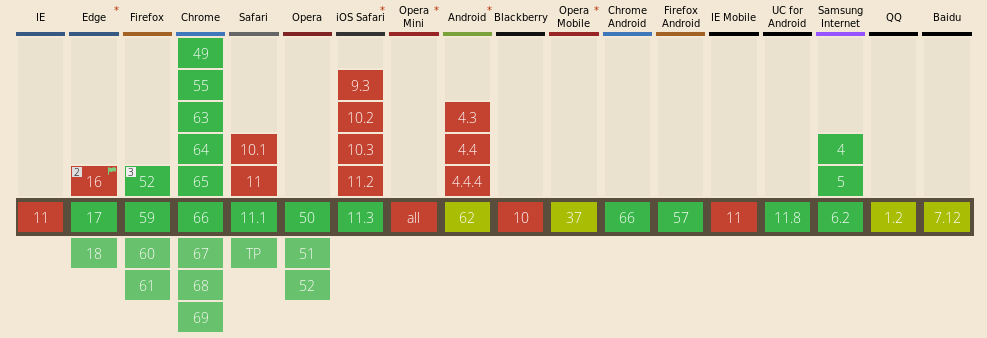
\includegraphics[width=1\textwidth]{ServiceWorker_all}
	\grayRule
	\caption[Browserkompatibilität für Service Worker]{Browserkompatibilität für Service Worker, Quelle: ~\cite{caniuse-sw}}
	\label{fig:serviceworker}
\end{figure}
%
Mit dem Service Worker können, wie mit dem App Cache, statische Ressourcen sofort beim ersten Besuch der Seite im Cache gespeichert werden. Es lässt sich hierbei unterscheiden, ob die Daten vor der ersten Verwendung, oder später im Cache gespeichert werden sollen. Für den ersten Fall eignen sich statische Inhalte wie Schriften oder JavaScript--Dateien, für den zweiten größere Ressourcen, die nicht sofort benötigt werden.\\
Zusätzlich bietet der Service Worker die Möglichkeit, auf Interaktionen zu reagieren. Den NutzerInnen kann angeboten werden, bestimmte Inhalte der Seite, wie zum Beispiel ein Video, später bzw. offline anzuschauen. Diese werden dann im Cache gespeichert und sind somit offline verfügbar.
Service Worker erlauben außerdem den Zugriff auf Push-Benachrichtigungen und das Background Sync \gls{API}. Die Hintergrundsynchronisation kann einmalig oder in festgelegten Intervallen stattfinden und ist besonders für nicht dringende Aktualisierungen wertvoll~\cite{offline_cookbook}.
%
% Browser
%
\sub{Speichern der generierten Daten}
Um NutzerInnenspezifische Daten offline verfügbar zu machen können sie im Browser gespeichert werden. Einige Methoden hierfür werden im Folgenden erläutert.
%
\subsub{Web Storage}
Das Web Storage \gls{API} ist ein Web-Standard, mit dessen Hilfe Daten als Schlüssel / Wert Paare im Browser gespeichert werden können. Es wird, wie Abbildung \ref{fig:webStorage} zeigt, von allen Browsern, bis auf den Opera Mini unterstützt. Opera Mini speichert grundsätzlich keine Daten, weswegen dieser Browser in den nachfolgenden Bildern mit Rot markiert ist.
Web Storage umfasst zwei Mechanismen, den SessionStorage und den LocalStorage.\\
Der SessionStorage existiert nur so lange das Browserfenster geöffnet ist.
Das heißt, dass alle Daten die im SessionStorage gespeichert werden, nicht mehr existieren sobald der Browser oder das Browserfenster geschlossen wird.
Daten die hingegen im LocalStorage gespeichert sind, existieren dort solange, bis der Browser Cache geleert wird~\cite{webstorage}.
\begin{figure}[H]
	\centering
	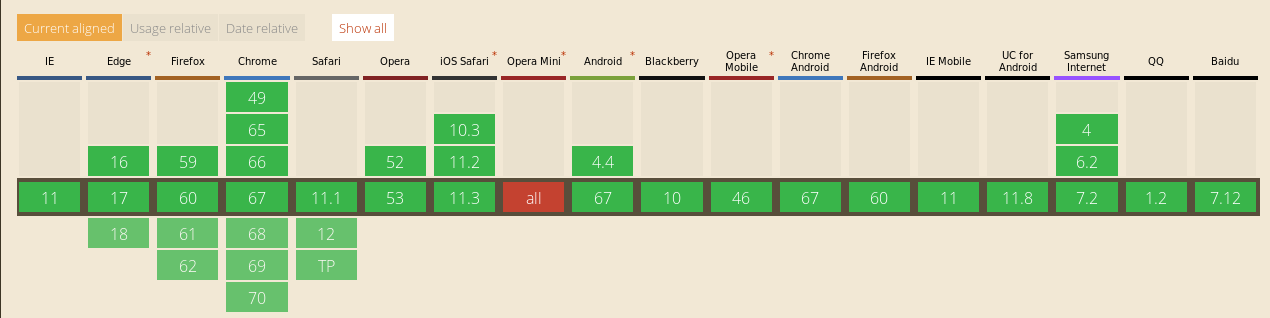
\includegraphics[width=\textwidth]{webStorage}
	\grayRule
	\caption[Browserkompatibilität für Web Storage]{Browserkompatibilität für Web Storage, Quelle: ~\cite{caniuse-ws}}
	\label{fig:webStorage}
\end{figure}
Der von den Browsern freigegebene Cache-Space für Web Storage variiert, ist aber meist auf 10 MB begrenzt.
Der größte Nachteil ist wohl, dass Web Storage synchron arbeitet und so andere Operationen, wie zum Beispiel das Rendern der Seite, blockieren kann ~\cite{webstorage-con}.
%
%
\subsub{Web SQL}
Eine andere Form der lokalen Speicherung im Browser ist die Web SQL Datenbank.
Sie hat ein asynchrones \gls{API} und unterstützt die grundlegenden SQL Abfragen. Web SQL sollte in den W3C Standards aufgenommen werden. Aus Mangel an unabhängigen Implementierungen wie z.B. eine andere \gls{DB} als SQLite im Backend, wurde es abgelehnt~\cite{websql}.\\
Das Web SQL \gls{API} wird nur von den Webkit--Browsern unterstützt, also nicht von Firefox, dem Internet Explorer oder dessen neueren Variante Edge~\cite{caniuse-websql}.
%
%
\subsub{IndexedDB}
IndexedDB ist eine weitere Variante der clientseitigen Datenspeicherung. Die auf Java"-Script basierende, objektorientierte Datenbank erlaubt neben dem Speichern von größeren Datenmengen in Form von Objekten auch das Speichern von Dateien. Durch die Verwendung von Indizes lassen sich Objekte schnell speichern und finden. Das asynchrone \gls{API} erlaubt Datenbankabfragen, die keinen anderen Prozess blockieren~\cite{idb}.
\begin{figure}[H]
	\centering
	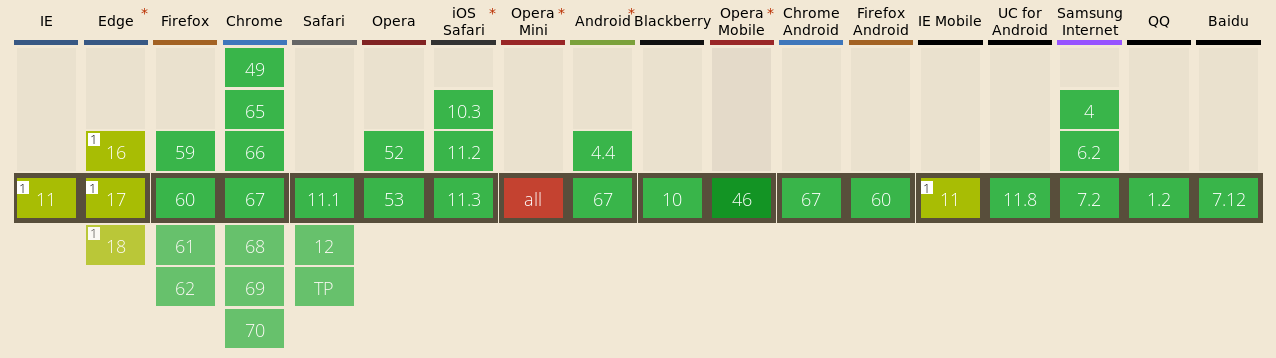
\includegraphics[width=\textwidth]{indexedDB}
	\grayRule
	\caption[Browserkompatibilität für IndexedDB]{Browserkompatibilität für IndexedDB, Quelle: ~\cite{caniuse-idb}}
	\label{fig:indexedDB}
\end{figure}
Wie in Abbildung \ref{fig:indexedDB} zu sehen ist, wird IndexedDB von allen gängigen Browsern unterstützt. 
%
\subsub{IndexedDB 2.0}
Im Januar 2018 wurde die zweite Version des IndexedDB \glspl{API} zur W3C Spezifikation hinzugefügt. Es erweitert die erste Verion um Funktionalität und verbessert die Performance~\cite{idb2}.
Die Aktualität dieser Spezifikation spiegelt sich in der Browserunterstützung wider. Die \autoref{fig:indexedDB2} zeigt, dass die zweite Version nur von den gängigen Desktopbrowsern und einigen mobilen Browsern unterstützt wird. Die IndexedDB 2.0 Unterstüzung in Edge wird von Microsoft geplant~\cite{edge}.
\begin{figure}[H]
	\centering
	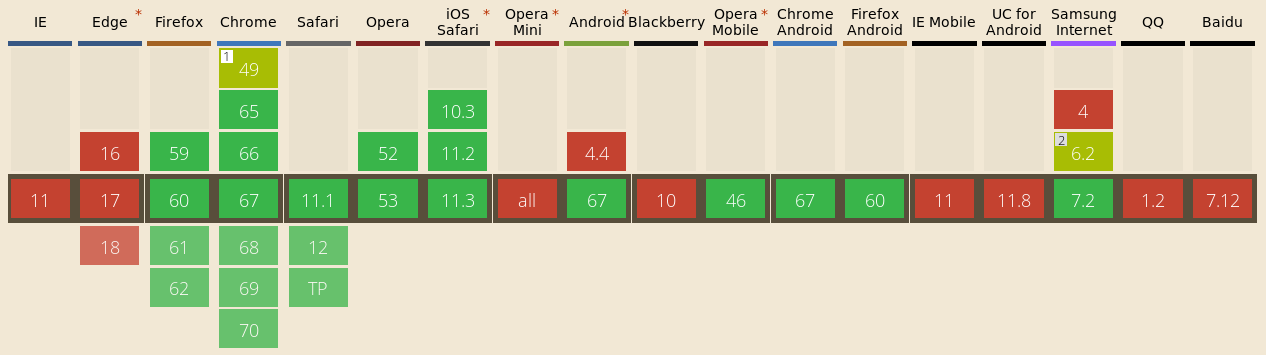
\includegraphics[width=\textwidth]{indexedDB2}
	\grayRule
	\caption[Browserkompatibilität für IndexedDB 2.0]{Browserkompatibilität für IndexedDB 2.0, Quelle: ~\cite{caniuse-idb}}
	\label{fig:indexedDB2}
\end{figure}
IndexedDB wird stetig weiterentwickelt und es gibt bereits einen Spezifikationsentwurf für die dritte Version~\cite{idb3}. 
%
% Sync
%
\sub{Datenbanksynchronisation}
\todo{ich weiß nicht ob das die richtige Stelle ist, Couch vorzustellen...}\\
Im Allgemeinen ist ein Synchronisationsprotokoll die Möglichkeit für zwei Partenen, beispielsweise Client und Server, den Zustand voneinander zu kennen. Der Client schickt seine Daten an den Server und umgekehrt, Konflikte werden gelöst, solange bis beide Parteien denselben Zustand haben.
Leider sind Synchronisationsprotokolle schwer zu implementieren und führen häufig zu einem frustrierenden Ergebnis: Dokumente oder Fotos werden nicht repliziert, es gibt doppelte oder verlorene Daten und alle möglichen Arten von Fehlverhalten bei kollaborativen Anwendungen.\\
CouchDB hat ein intergiertes \hyperref[chap:replication]{Replikationsprotokoll}, das diesen Teil behandelt.  
%
% Couch
%
\subsub{\label{chap:couch}CouchDB}
Apache CouchDB\tm ist ein \gls{DBMS} das seit 2005 als freie Software entwickelt wird. Die dokumentenorientierte \gls{DB} funktioniert sowohl als einzelne Instanz, als auch im Cluster, in dem ein Datenbanksserver auf einer beliebig großen Anzahl an Servern oder Virtuellen Masschinen ausgeführt werden kann.\\
% So kann die Datenschicht beliebig skaliert werden, um die Anforderungen vieler BenutzerInnen zu erfüllen.
CouchDB verwendet das \gls{HTTP}--Protokoll und \gls{JSON} als Datenformat, weswegen es mit jeder Webfähigen Anwendung kompatibel ist. CouchDB wird über ein \gls{REST}ful \gls{HTTP} \gls{API} angesprochen. So können Daten über die für den \gls{REST}ful Services standardisierten Methoden wie zum Beispiel GET, POST, PUT, DELETE abgerufen oder manipuliert werden.\\\\
Das implementierte Replikationsmodell erlaubt die Synchronisation bzw. bidirektionale Replikation zu verschiedenen Geräten, was das besondere Merkmal von CouchDB ist. 
Die genaue Funktionsweise des Protokolls wird in \autoref{chap:replication} detailliert beschrieben.\\
Dieses Protokoll ist die Grundlage für Offline First Anwendungen.
Dank des Replikations--\gls{API} kann kann sich eine CouchDB kontinuierlich und eigenständig mit einer anderen Datenbank die dasselbe Protokoll implementiert, synchronisieren.
Wenn Konflikte auftreten, beispielsweise durch gleichzeitiges Bearbeiten eines Dokuments von zwei Personen ohne Netzwerkverbindung, werden diese als solche markiert, jedoch nicht von selbst aufgelöst~\cite{couch}. Die Lösung der Konflikte muss in der Anwendung implementiert sein.
So kann gewährleistet werden, dass keinerlei Daten verloren gehen.\\\\
CouchDB ist für Server konzipiert. Für Browser gibt es \hyperref[chap:pouch]{PouchDB} und für native iOS- und Android--\glspl{App} wurde Couchbase Lite entwickelt.
Des Weiteren gibt es noch die Datenbanken Couchbase und Cloudant.
Alle verwenden das CouchDB Replikationsprotokoll und können Daten miteinander replizieren und~\cite{couch}.
%
% Pouch
%
\subsub{\label{chap:pouch}PouchDB}
Als Ergänzung zu CouchDB kann PouchDB verwendet werden. PouchDB ist die Java"-Script Implementierung von CouchDB.
Sie ist quelloffen und wurde so konzipiert, dass sie in allen modernen Browsers läuft. Dort ermöglicht PouchDB es Daten zu persistieren, sodass sowohl offline als auch online verfügbar sind.
PouchDB speichert die Daten in IndexedDB und stellt für das Abrufen und Manipulieren derer ein einheitliches \gls{API} zur Verfügung.\\
Sind die Daten einmal offline gespeichert können sie, dank des CouchDB Replikationsprotokolls, sobald die Awendung wieder online ist mit CouchDB kompatiblen Servern synchronisiert werden~\cite{pouch}.
% %
% % PWA
% %
% \sub{\label{sub:pwa}Progressive Web Apps \todo{raus?}}
% \Gls{PWA} ist eine Bezeichnung für eine mobil nutzbare Webseite, die eine Brücke zwischen der nativen
% Applikation und einer Webseite schlägt.
% Der Begriff \gls{PWA} wurde im Jahr 2015  von Alex Russel und seiner Frau Frances Berriman geprägt.
% Dieser beschreibt Webseiten, die die positiven Funktionen von nativen Applikationen mitbringen, aber statt über App Stores installiert zu werden, im Webbrowser existieren. Die Webseiteninhalte sind ohne die Installation sofort und jederzeit für die NutzerInnen abrufbar. Schon beim zweiten Besuch der Webseite ist die Ladezeit der Daten verkürzt und sie ist offline, oder auch bei schlechter Internetverbindung nutzbar. Nach mehrmaligem Aufruf kann die \gls{PWA} über den Browser installiert und zum Startbildschirm hinzugefügt werden. Russel und Berriman legen folgende Einenschaften einer \gls{PWA} fest:
% \begin{itemize}
% 	\item Responsive %to fit any form factor
% 	\item Connectivity independen]% Progressively-enhanced with Service Workers to let them work offline
% 	\item App-like-interaction]% Adopt a Shell + Content application model to create appy navigations \& interactions
% 	\item Fresh %Transparently always up-to-date thanks to the Service Worker update process
% 	\item Safe %Served via TLS (a Service Worker requirement) to prevent snooping
% 	\item Discoverable %Are identifiable as “applications” thanks to W3C Manifests and Service Worker registration scope a llowing search engines to find them
% 	\item Re-engageable %Can access the re-engagement UIs of the OS; e.g. Push Notifications
% 	\item Installable %to the home screen through browser-provided prompts, allowing users to “keep” apps they find most useful without the hassle of an app store
% 	\item Linkable %meaning they’re zero-friction, zero-install, and easy to share. The social power of URLs matters.
% \end{itemize}
% \todo{Näher erläutern?}~\cite{pwa}.

%
% Konflikte
%
\section{WIP Konfliktmanagementstrategien}
Diese Arbeit untersucht die Konfliktmanagementstrategien offlinefähiger Systeme. Nachdem in \autoref{chap:offlinefirst} beschrieben wurde was eine Anwendung offlinefähig macht, wird in diesem Abschnitt definiert was ein Konflikt ist und wie er entsteht.
\sub{\label{sec:conflict}Konflikte}
% 1. Definition
Als Konflikt wird die Situation bezeichnet, in der verschiedene Versionen des gleichen Dokuments auf mehreren Geräten oder Datenbanken gespeichert sind (vgl. ~\cite{couchDB} S. 153).
Konflikte gehören in verteilten Systemen zur Realität und lassen sich nicht vermeiden.
Ein verteiltes System ist per Definition ein Zusammenschluss unabhängiger Computer, die sich für die NutzerInnen als ein einziges System präsentieren (vgl. ~\cite{tanenbaum} S. 2).
Einfacher gesagt, besteht ein verteiltes System, sobald zwei oder mehrere Computer über das Netzwerk miteinander verbunden sind.
Die spezielle Eigenschaft von Netzwerken ist jedoch, dass die Verbindung jederzeit abbrechen kann.
Gareth Wilson beschreibt in seinem Artikel die acht Irrtümer zur verteilten Datenverarbeitung ~\cite{fallacies}:
\begin{enumerate}
  \item Das Netzwerk ist zuverlässig
  \item Die \gls{Latenz}zeit ist gleich null
  \item Die Bandbreite ist unendlich
  \item Das Netzwerk ist (informations)sicher
  \item Die Netzwerkstruktur wird sich nicht ändern
  \item Es gibt eineN AdministratorIn
  \item Die Datentransportkosten sind gleich null
  \item Das Netzwerk ist homogen
\end{enumerate}
Aus diesen irrtümlichen Annahmen über das Netzwerk ergeben sich Fehlerszenarien. So kann es passieren, dass der zweite Computer entweder sehr weit entfernt, sehr beschäftigt oder ausgeschaltet ist. Diese Fehlerszenarien können dazu führen, dass ein Konflikt entsteht.
Anhand des folgenden Beispiels wird ein mögliches Fehlerszenario für den Fall des unzuverlässigen Netzwerks aufgegriffen.\\
%
Zwei Personen treffen sich im Zug und verstehen sich auf Anhieb sehr gut. Person A, nennen wir sie Amilia, gibt Person B, nennen wir sie Rory, ihre Telefonnummer. Der Zug fährt durch einen Tunnel und das Netzwerk bricht ab, als Rory Amilias Nummer in sein Adressbuch, das in Form einer \gls{App} auf seinem Laptop gespeichert ist, schreibt.
Amilia diktiert ihre Telefonnummer falsch, mit einem Zahlendreher, weil sie die Nummer noch nicht lange hat.
Zur Sicherheit schickt Amilia Rory ihre Nummer zusätzlich per E-Mail. Rory schaltet seinen Laptop aus, weil er sich mit Amilia unterhalten möchte.
Am Abend ist Rory zu Hause angekommen und er speichert Amilias Nummer aus der E-Mail in seinem Adressbuch auf seinem stationären Desktop PC.
Jetzt gibt es Amilias Telefonnummer mit unterschiedlichen Informationen in Rorys Adressbuch auf verschiedenen Geräten.
Wenn Rory am nächsten Tag seinen Laptop startet und das Adressbuch sich mit dem auf dem PC synchronisiert, entsteht ein Konflikt.
Es gibt zwei unterschiedliche Versionen von Amilias Telefonnummer auf Rorys Geräten.\\\\
% Die korrekte Telefonnummer vom stationären PC befindet sich bereits auf dem Server und wird nun, da sich jetzt das Adressbuch auf dem Laptop mit dem Server synchronisiert, von der Nummer mit dem Zahlendreher überschrieben.
% Die falsche Telefonnummer wird gespeichert und die richtige ist verloren.\\\\
%
%
Konflikte sind in zwei Kategorien einzuteilen. Es gibt solche, die vom System selbst gelöst werden können und solche, die eine spezielle Behandlung brauchen.
Gibt es eine gleichzeitige Änderung an unterschiedlichen Stellen eines Dokuments, muss das kein Problem darstellen.
Das Dokument kann beide Aktualisierungen erhalten, indem die Änderungen zusammengefügt werden.
Diese Prozedur wird \it{merge} genannt und ist durch Systeme wie Git\footnote{git steht unter \url{https://git-scm.com/downloads} zum Download bereit}, einer Software zur verteilten Versionsverwaltung, den meisten EntwicklerInnnen bekannt. Diese Art Konflikt kann selbstständig vom System gelöst werden.\\

Die Konflikte, die durch verschiedene Änderungen an ein und derselben Stelle des Dokuments entstehen, benötigen eine aufwändigere Behandlung.
Es muss festgestellt werden, welche Version die korrekte ist und gespeichert werden soll.
Die Wiederherstellung der Datenkonsistenz bei Konflikten kann dazu führen, dass einige oder alle Aktualisierungen ganz oder teilweise gelöscht werden.
Zur Lösung dieses Problems wurden verschiedene Managementstrategien entworfen, die im Folgenden vorgestellt werden.
%
%
% \begin{description}[leftmargin=0.5cm,style=nextline]
% 	\item[1. Das Netzwerk ist zuverlässig] ~ Der Strom kann ausfallen oder Glasfaserkabel können kaputt sein --- Das Netzwerk ist nicht zuverlässig.
% 	\item[2. Die \gls{Latenz} ist gleich null] ~ Glasfaserkabel werden durch Mikrowellen (oder andere Technologien) ersetzt um Millisekunden an Zeit zu sparen. Das würde nicht passieren, wäre die \gls{Latenz} bei null. Es dauert nun mal eine gewisse Zeit(ms) wenn ein Signal eine (geografisch)weite Strecke zurücklegen muss --- Die Latenz ist nicht gleich null.
% 	\item[3. Die \gls{Bandbreite} ist unendlich] ~ Daten können nicht schneller fließen als die Komponenten die sie verarbeiten (\gls{Middleware}, Datenbank \ldots) --- Die Bandbreite ist nicht unendlich.
% 	\item[4. Das Netzwerk ist sicher] ~ Der \sc{Heartbeat-bug}\footnote{\url{http://heartbleed.com/} -- Zugriff: 07.04.2018}, der im Jahr 2014 behoben wurde und die Sicherheitslücke im ICE-\gls{WLAN} im Jahr 2016\footnote{\url{https://netzpolitik.org/2016/datenschutz-im-zug-deutsche-bahn-will-sicherheitsluecke-in-neuem-ice-wlan-schliessen/} -- Zugriff: 07.04.2018} sind nur zwei Beispiele die zeigen, dass das Netzwerk nicht sicher ist.
% 	\item[5. Die Netzwerkstruktur wird sich nicht ändern] ~ Eine Datenbank kann beispielsweise über mehrere Server verteilt sein, die (teilweise) voneinander abhängig sind. Ein Server mit Abhängigkeiten kann ausfallen, es kann eine Aktualisierung für einen anderen Server geben --- die Struktur ändert sich.
% 	\item[5. Die Netzwerkstruktur wird sich nicht ändern] ~ Eine Datenbank kann beispielsweise über mehrere Server verteilt sein, die (teilweise) voneinander abhängig sind. Ein Server mit Abhängigkeiten kann ausfallen, es kann eine Aktualisierung für einen anderen Server geben --- die Struktur ändert sich.
% 	\item[6. Es gibt eineN AdministratorIn] ~ Es kann beliebig viele AdministratorInnen geben.
% 	\item[7. Die Datentransportkosten sind gleich null] ~ Netflix bezahlte anfang 2014 diversen InternetanbieterInnen dafür, dass Netflix KundInnen bevorzugten Internetzugang haben.
% 	\item[8. Das Netzwerk ist homogen] ~ Es gibt verschiedene Arten von Netzwer: 3G, 4G, LTE, WiFi. Wird beeinflusst durch Hardware (Smartphone, Tablet, PC, Laptop, Router \ldots)~\cite{fallacies}
% \end{description}

%
\sub{WIP Spätere Konsistenz}
\todo{Das muss noch woanders hin. oder raus}\\
Das \gls{CAP} Theorem, veranschaulicht in \autoref{fig:cap}, besagt, dass jedes System mit dem Daten über das Netzwerk gesendet werden, nur zwei von den drei möglichen Eigenschaften, Konsistenz, Verfügbarkeit und Partitionstoleranz, garantieren kann.
Konsitzenz der gespeicherten Daten bedeutet, es muss sichergestellt werden dass nach Abschluss der Transaktion auch alle Replikate des manipulierten Datensatzes aktualisiert werden. Der Datensatz ist in jeder Datenbank identisch.
%
\begin{figure}[H]
  \centering
  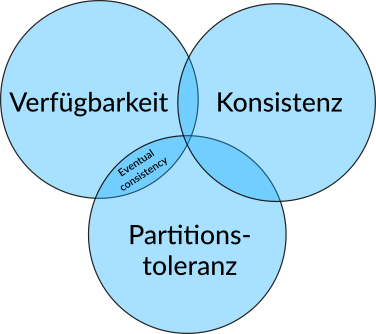
\includegraphics[width=0.6\textwidth]{cap}
  \grayRule
  \caption{Das CAP Theorem}
  \label{fig:cap}
\end{figure}
%
Das System ist besitzt eine hohe Verfügbarkeit wenn alle Anfragen an das System stets beantwortet werden. Die Verfügbarkeit ist gering, wenn die Antwortzeiten des Systems lang sind.
Partitionstoleranz ist gleichzusetzen mit Ausfalltoleranz. Die Datenbank kann auf mehreren Servern verteilt sein. Trotzdem ein Server oder eine Partition ausfällt, kann das System weiterhin funktionieren.\\
Eventual Consistency kommt häufig bei verteilten Datenbanken zur Anwendung und stellt die Konsitenz der Daten nach einem gewissen Zeitfenster sicher (vgl. ~\cite{couchDB} S. 11 ff.). 
% Wenn Verfügbarkeit Priorität hat, können wir Clients die Daten zunächst auf einen Knoten schreiben lassen, ohne darauf zu warten, dass die anderen Knoten synchronisiert werden.
% Wenn die Datenbank weiß, wie sie mit dieser Situation umzugehen hat, sind die Daten irgendwann „letztendlich konsistent“ — allerdings unter Aufgabe der Hochverfügbarkeit der Daten.
% Für viele Anwendungen ist das ein erstaunlich guter Kompromiss.
%
% Couch Pouch
%
%
\sub{Last-Write-Wins}
Der \gls{LWW} Ansatz geht davon aus, dass Schreibvorgänge immer in der richtigen Reihenfolge ausgeführt werden. Der letzte an die Datenbank gesendete Schreibvorgang wird als korrekt angenommen.
%Konflikte werden bei dieser Strategie ignoriert
Diese Strategie ist leicht zu implementieren da lediglich festgestellt werden muss welche Manipulation die neuere ist, was durch die Vergabe eines Zeitstempels problemlos zu errechnen ist ~\cite{lww}.\\
%\quote{When multiple updates are applied to the same column, Cassandra uses clientprovided timestamps to resolve conflicts}
%
\sub{WIP Operational Transformation}
\note{siehe woot}\\
\gls{OT} ist eine weit verbreitete Technologie zur Unterstützung von Funktionalitäten in \gls{kollaborativ}er Software. Sie stammt aus einer im Jahre 1989 veröffentlichten Forschungsarbeit und wurde ursprünglich nur für die gemeinsame Bearbeitung von Klartext-Dokumenten entwickelt~\cite{ot_paper}. Später ermöglichte weitere Forschung \gls{OT} durch Unterstützung von \textit{Sperrungen, Konfliktlösungen, Benachrichtigungen, Bearbeitung von Baumstrukturierten Dokumenten, ...} zu verbessern und erweitern. Im Jahr 2009: Google Wave, Google Docs\\
%
%
\Gls{kollaborativ}e Systeme, die \gls{OT} verwenden, benutzen normalerweise den replizierten Dokumentenspeicher. Das heißt jeder \b{Client} verfügt über eine eigene Kopie des Dokuments.
Jede Änderung an einem freigegebenen Dokument wird als Operation dargestellt. Operationen sind Repräsentationen von Änderungen an einem Dokument. (Beispielsweise: Füge 'Hello world!' an Position 0 in das Textdokument ein).  Eine Operation zeichnet im Wesentlichen den Unterschied zwischen einer und der nachfolgenden Version eines Dokuments auf. Die Anwendung einer Operation auf das aktuelle Dokument führt zu einem neuen Dokumentstatus.
Die Operationen erfolgen auf lokalen Kopie und die Änderungen werdenn an alle anderen \b{Clients} weitergegeben.  Wenn ein \b{Client} die Änderungen von einem anderen \b{Client} empfängt, werden die Änderungen normalerweise \b{vor} ihrer Ausführung transformiert.
\highlight{Die Transformation stellt sicher, dass anwendungsabhängige Konsistenzkriterien (Invarianten) von allen Standorten gepflegt werden. }\\
Es gibt die Operationen \b{Einfügen}\\
Das Einfügen besteht aus dem eingefügten Text und dessen Position im Dokument (\tt{insert('h', 0)}).
Für die Position kann ein Koordinatensystem ermittelt werden (Zeilennummer: Position in Zeile oder einfacher: Dokument wie eine Folge von Zeichen behandeln, also einfach einen nullbasierten Index vergeben.)\\
und \b{Löschen}\\
Löschen(5,6) = löscht 5 Zeichen, beginnend bei Position 6.
Mehr benötigt man nicht, denn update = delete \& insert\\\\
Um gleichzeitige Operationen zu behandeln, gibt es eine Funktion (normalerweise \texttt{Transform} genannt), die zwei Operationen übernimmt, die auf denselben Dokumentstatus angewendet wurden (aber auf verschiedenen Clients).
Daraus wird eine neue Operation berechnet, die nach der zweiten Operation angewendet werden kann. Diese behält die erste beabsichtigte Änderung der Operation.
Des Weiteren unterstützt \gls{OT} Operationen wie \tt{update}, \tt{point}, \tt{lock}.
\paragraph{Beispiel}:
Benutzer A fügt an Position 12 das Zeichen 'A' ein
Benutzer B fügt am Anfang des Dokuments ein 'B' ein.
Die konkurrierenden Operationen sind daher Einfügen (12, 'A') und Einfügen (0, 'B').
Wenn wir die Operation von B einfach an Client A senden und dort anwenden würden, gäbe es ein Problem.
Aber wenn die Operation von A an B gesendet, und angewandt wird nachdem Operation B angewandt wurde ist, würde das Zeichen 'A' eine Position zu weit links von der korrekten Position eingefügt werden.
Dokumentstatus A und Dokumentstatus B sind nicht identisch.\\
Daher muss A's \tt{insert(12, 'A')} gegen die Operation von B transformiert werden. So wird berücksichtigt, dass B ein Zeichen vor der Position 12 eingefügt hat (die die Operation \tt{insert(13, 'A')} erzeugt.)\\
Diese neue Operation kann auf Dokument B nach B's Operation angewandt werden.
Die Grundidee von \gls{OT} besteht darin, die Parameter einer Editieroperation gemäß den Auswirkungen \b{zuvor ausgeführter} konkurrierender Operationen anzupassen, so dass die transformierte Operation die korrekte Wirkung erzielen und die Dokumentenkonsistenz aufrechterhalten kann.
%
% Kritik
%
False-Tie puzzle? \it{A Generic Operation Transformation Scheme for Consistency Maintenance in Real-time Cooperative Editing Systems} und \it{Achieving convergence, causality-preservation, and intention-preservation in real-time cooperative editing systems}\\\\
Während der klassische OT-Ansatz, Operationen durch ihre Versätze im Text zu definieren, einfach und natürlich zu sein scheint, werfen real verteilte Systeme ernsthafte Probleme auf. Nämlich, dass sich die Operationen mit endlicher Geschwindigkeit fortpflanzen, die Zustände der TeilnehmerInnen sind oft verschieden, so dass die resultierenden Kombinationen von Zuständen und Operationen extrem schwer vorherzusehen und zu verstehen sind.
Wie Li und Li es ausdrückten: ``Aufgrund der Notwendigkeit, eine komplizierte Fallabdeckung in Betracht zu ziehen, sind formale Beweise sehr kompliziert und fehleranfällig, selbst für OT-Algorithmen, die nur zwei charakteristische Primitive behandeln (Einfügen und Löschen)``~\cite{ot-critic}.\\
Damit OT funktioniert, muss jede einzelne Änderung an den Daten erfasst werden: ``Einen Schnappschuss des Zustands zu erhalten, ist normalerweise trivial, aber das Erfassen von Bearbeitungen ist eine ganz andere Sache. [...] Der Reichtum moderner Benutzerschnittstellen kann dies problematisch machen, besonders in einer browserbasierten Umgebung`` ~\cite{diff_sync}.
%
\sub{WIP Conflict-Free Replicated Data Type}
%
% CRDT
%
Ein \gls{CRDT} ist eine spezielle Datenstruktur die in verteilten Systemen auf mehreren Geräten repliziert werden kann. Jede Operation wird an alle Replikate gesendet. Jedes Replikat wendet alle ankommenden Aktualisierungen an und ein Algorithmus löst alle konfliktbehafteten Aktualisierungen auf, wodurch sichergestellt ist, dass Konflikte gar nicht erst auftreten~\cite{crdt_shapiro}. Eine Synchronisation ist nicht notwendig, da die Aktualisierung sofort ausgeführt wird ~\cite{crdt_shapiro2}.\\\\
%
Es gibt zwei Konzepte bei Replikationsmodellen mit \glspl{CRDT}: den zusandsbasierten und den operationsbasierten Ansatz.
%In seinem Vortrag beschreibt Marc Shapiro die Funktionsweisen beider Ansätze und geht auf die Unterschiede, Vor- und Nachteile ein.
%Bei operationsbasierten \glspl{CRDT} muss sichergestellt werden, dass die Operationen nicht verloren gehen oder dupliziert werden wenn sie zu den anderen Replikaten übertragen werden.
%Zustandsbasierte \glspl{CRDT} haben den Nachteil, dass der gesamte Zustand, statt nur der Operation und die sich ändernden Abschnitte, zu den anderen Replikaten übertragen werden muss.
%
\subsub{Zustandbasierter Ansatz}
Wenn ein Replikat eine Aktualisierung von einem Client empfängt, wird es zuerst auf den lokalen Status angewandt.
Dann sendet es etappenweise eine Kopie des eigenen, aktualisierten Status an andere Replikate im System.
Wenn ein Replikat den Status eines anderen Replikats empfängt, führt es mit einer \tt{merge} Funktion den empfangenen Status mit dem lokalen zusammen.
Entsprechend sendet dieses Replikat gelegentlich auch seinen Status an ein anderes Replikat, sodass jede Aktualisierung schließlich alle Replikate im System erreicht ~\cite{crdt_shapiro2}.
Die folgende Abbildung stellt eine zustandsbasierte Replikation mit drei Geräten dar.
%
\begin{figure}[H]
  \centering
  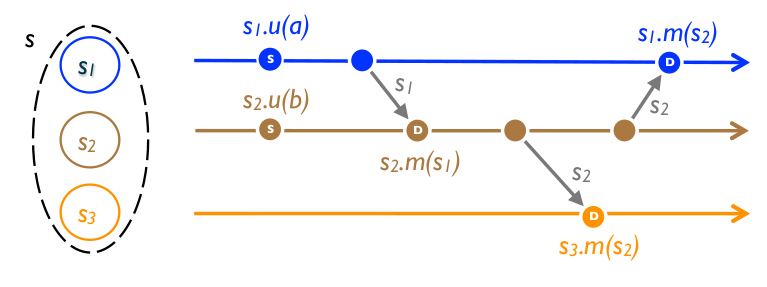
\includegraphics[width=0.8\textwidth]{crdt-state}
  \grayRule
  \caption[Replikation von zustandsbasierten \glspl{CRDT}]{Replikation von zustandsbasierten \glspl{CRDT}, Quelle: ~\cite{crdt_shapiro2}}
  \label{fig:crdt-state}
\end{figure}
%
Die drei Kreise auf der linken Seite repräsentieren drei identische Datensätze auf drei Geräten. Die Datensätze \it{S1} und \it{S2} werden zeitgleich mit unterschiedlichem Kontent aktualisiert.
Kurz darauf, weiter rechts im Bild, sendet \it{S1} seinen neuen Status an \it{S2}.
\it{S2} führt die beiden Status, den von \it{S1} empfangenen und den eigenen, aktualisierten, in der \tt{merge} Funktion $m$ zusammen.
Dann schickt es den eigenen, neuen Status an \it{S3} und \it{S1}, welche ebenfalls den empfangenen mit dem eigenen Status zusammenführen. Beide Aktualisierungen haben nun alle Geräte erreicht und alle Daten sind identisch.\\\\
%
Damit die Replikation konfliktfrei funktioniert müssen einige Voraussetzungen erfüllt sein.
Der Status, den ein \gls{CRDT} hat muss ein Semi--Gitter, also eine geordnete Menge abbilden.
Die Aktualisierungen müssen zunehmend sein, ein Status kann beispielsweise eine Zahl sein und die Aktualisierung ist die Operation die sie inkrementiert.
Die \tt{merge} Funktion muss die kleinste obere Grenze der letzten Aktualisierung berechnen.
Nur wenn ein Objekt diese Eigenschaften erfüllt, ist es dem \gls{CRDT} zugehörig ~\cite{crdt_shapiro2}
%
%
%
\subsub{Operationsbasierter Ansatz}
Wenn ein Replikat eine Aktualisierung von einem Client empfängt, wird es ebenfalls zuerst auf den lokalen Status angewandt.
Im Gegensatz zum zustandsbasiertem Ansatz wird nicht der gesamte Status des Replikats gesendet, sondern nur der Aktualisierungsvorgang.
Ein weiterer Unterschied ist das Fehlen der \tt{merge} Funktion. Statt ihrer gibt es im operationsbasierten Ansatz zwei \tt{update} Methoden: eine vorbereitende Aktualisierungsfunktionen und eine ausführende. Erstere wird auf dem Replikat angewandt, umgehend gefolgt von der zweiten.
Über ein Kommunikationsprotokoll wird die Aktualisierung an alle anderen Replikas asynchron versendet.
Über das Protokoll wird sichergestellt, dass die Nachricht nur einmal überliefert wird.
Die restlichen Replikas wenden die Operation mit der ausführenden Aktualisierungsmethode auf sich an~\cite{crdt_shapiro2}.
Die folgende Abbildung stellt eine operationsbasierte Replikation mit drei Geräten dar.
%
\begin{figure}[H]
  \centering
  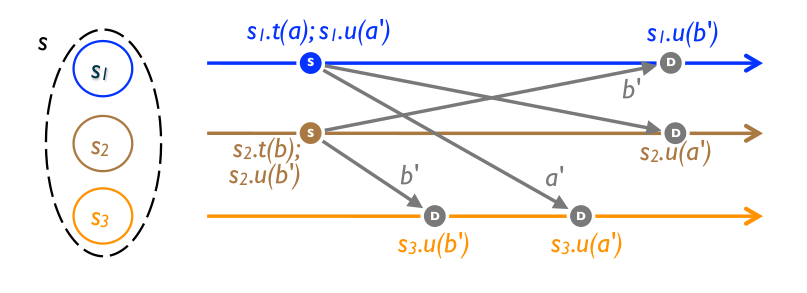
\includegraphics[width=0.8\textwidth]{crdt-op}
  \grayRule
  \caption[Replikation von Operationsbasierten \gls{CRDT}]{Replikation von Operationsbasierten \glspl{CRDT}, Quelle: ~\cite{crdt_shapiro2}}
  \label{fig:crdt-op}
\end{figure}
%
Die drei Kreise auf der linken Seite repräsentieren drei identische Datensätze auf drei Geräten. Die Datensätze \it{S1} und \it{S2} werden zeitgleich mit unterschiedlichem Kontent aktualisiert.
Sowohl \it{S1} also auch \it{S2} wenden die vorbereitende Aktualisierungsmethode $t$ auf sich an.
Dann, mit dessen Ergebnis, die ausführende $u$.
Sofort senden beide Relikas die Aktualisierung an alle anderen, welche ebenfalls die ausführende Aktualisierungsmethode $u$ auf sich anwenden.\\\\
Die Voraussetzung für eine konfliktfreie Replikation sind hier kommuntative Aktualisierungen.
%Wenn $s$ der Status ist und $u$ die Aktualisierungsmethode, muss $s \bullet u \bullet u' \equiv s \bullet u' \bullet u$ gelten.
Nur so spielt die Reihenfolge in der die Aktualisierungen bei den Replikaten ankommen, keine Rolle -- das Ergebnis ist dasselbe ~\cite{crdt_shapiro2}.\\\\
Umgesetzte \glspl{CRDT} sind zum Beispiel Counter, ein Datenobjekt das zum Zählen verwendet wird. Es gibt einen, der nur hochzählen kann und eine andere Variante die auch die Subtraktion unterstützt.
Weitere \glspl{CRDT} sind Sets, eine Listenrepräsentation ohne Duplikate. Auch hier gibt es eine Variante mit der nur Daten hinzugefügt werden können und eine die auch das Entfernen der Daten erlaubt ~\cite{crdt_shapiro}.
%
%CRDTs befassen sich mit einem interessanten und grundlegendem Problem in verteilten Systemen, haben jedoch eine wichtige Einschränkung:
%"Da ein CRDT konstruktionsbedingt keinen Konsens verwendet, hat der Ansatz starke Einschränkungen; Dennoch sind einige interessante und nicht-triviale CRDTs bekannt" ~\cite{crdt_shapiro2}.
%Die Einschränkung ist, dass die CRDT-Adresse nur einen Teil des Problemraums betrifft, da nicht alle möglichen Aktualisierungsoperationen kommutativ sind und daher nicht alle Probleme in CRDTs umgewandelt werden können.
%
%Alas, everything in programming is trade-offs, so what do we trade for being able to have conflict-free data structures? Well, they are specialised data structures, like sets and counters, and not generic object representations like JSON, so we’ll have to buy into a whole world of these specialised data structures, and maybe we have hard time mapping our application objects to them. 
%
\sub{Differential Synchronization?}
%
\sub{\label{sec:replication}WIP Das CouchDB Replikationsmodell}
\hyperref[chap:couch]{CouchDB} ist ein quelloffenes, dokumentenorientiertes \gls{DBMS} mit einem integrierten Replikationsprotokoll.\\
Die Aufgabe der Replikation von CouchDB ist die nahtlose, direkte Datensynchronisation zweier oder mehrerer Datenbanken.
CouchDB verwendet Replikation um Änderungen an Dokumenten zwischen einzelnen Knoten zu synchronisieren.
%. These databases can live on the same server or on two different servers—CouchDB doesn’t make a distinction. If you change one copy of the database, replication will send these changes to the other copy. 
Hierbei werden nur die Dokumente übertragen, die neu sind oder sich geändert haben.
Die Replikation in CouchDB erfolgt schrittweise. Alle Änderungen an Dokumenten werden periodisch zwischen den Servern kopiert.
Wenn der Replikationsprozess unterbrochen wurde weil eine Datenbank keinen Internetzugang hat, haben zwei sich replizierende Datenbanken unterschiedliche Daten gespeichert -- einen inkosistenten Status.
Bei wieder bestehender Internetverbindung wird die Replikation erneut ausgelöst und CouchDB setzt an dem Punkt an dem es ausgefört hat, die Arbeit fort.\\\\
%
Das Besondere an CouchDB ist, dass es darauf ausgerichtet ist, Konflikte vernünftig zu behandeln statt anznehmen es träten keine auf.
Das interne Replikationssystem besitzt eine automatische Konflikterkennung und --lösung.\\
Wichtig für diesen Mechanismus sind die Revisionsnummern.
Dokumente werden mit Revisionsnummern versioniert. Mit jeder Aktualisierung bekommt es eine neue Revision, die neben der alten gespeichert wird (vgl. \cite{couchDB} S. 15ff \& S. 150ff). 
Eine Revisionsnummer in CouchDB kann wie folgt aussehen \tt{2-5560348cec1b08c3d53e1508b4a46868} und ist in zwei Bereiche zu teilen. Die Zahl vor dem \tt{-} erhöht sich mit jeder neuen Revision des Dokuments, also mit jeder Aktualisierung. Alles hinter dem Strich ist ein md5--\gls{Hash} aus dem Dokumenteninhalt, den Dateianhängen und dem \tt{\_deleted} Attribut\footnote{ Dokumente werden in CouchDB nicht ohne Weiteres gelöscht. Stattdessen werden sie als solches markiert.}. Jede Revision hat außerdem eine Liste von vorherigen Revisionen.\\\\
Hat ein Dokument durch gleichzeitiges Bearbeiten in zwei unterschiedlichen Datenbanken dieselbe Revisionsnumer, erkennt CouchDB den Konflikt und markiert indem das Dokument das Attribut \tt{\_conficts} mit dem Wert \tt{true} bekommt. Dann entscheidet CouchDB, welche Version gewinnt und welche verliert.
CouchDB wird nie zwei Versionen zusammenführen. Das muss in der Anwendung implementiert sein.
Die Entscheidung darüber, welche Version gewinnt erfolgt über den Längenvergleich der Revisionslisten. Die Version mit der längsten Liste aus vorherigen Revisionen gewinnt. Sind beide Listen gleich lang, gewinnt die Revision die laut alphabetischer Sortierung am größten ist.\\
Auch wenn CouchDB die gewinnende und die verlierende Revision festlegt, werden beide Versionen gespeichert. Die gewinnende Revision wird als letztes gespeichert, die verlierende davor. Diese Konfliktlösungsstrategie wird auf allen CouchDB Instanzen angewandt, weswegen dazu keine Internetverbindung notwendig ist. Dadurch, dass alle Instanzen denselben Algorithmus verwenden werden die Revisionen immer in identischer Reihenfolge gespeichert. Dadurch bleiben die Daten konsistent.\\
Jetzt kann im Entwicklungsprozess der Anwendung entschieden werden, wie mit den Konflikten umgegangen wird.
Es kann aus beiden Version eine festgelegt werden, die behalten wird oder es können beide zusammengeführt werden (vgl. \cite{couchDB} S. 153ff).
%
\subsub{Eventual Consistency}
\todo{Das muss noch woanders hin. oder raus}\\
Das \gls{CAP} Theorem, veranschaulicht in \autoref{fig:cap}, besagt, dass jedes System mit dem Daten über das Netzwerk gesendet werden, nur zwei von den drei möglichen Eigenschaften, Konsistenz, Verfügbarkeit und Partitionstoleranz, garantieren kann.
Konsitzenz der gespeicherten Daten bedeutet, es muss sichergestellt werden dass nach Abschluss der Transaktion auch alle Replikate des manipulierten Datensatzes aktualisiert werden. Der Datensatz ist in jeder Datenbank identisch.
%
\begin{figure}[H]
  \centering
  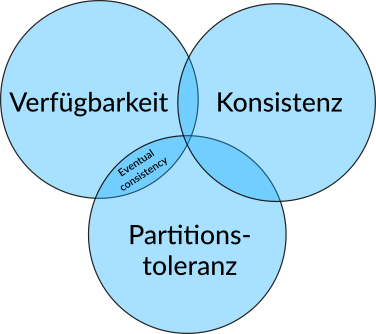
\includegraphics[width=0.6\textwidth]{cap}
  \grayRule
  \caption{Das CAP Theorem}
  \label{fig:cap}
\end{figure}
%
Das System ist besitzt eine hohe Verfügbarkeit wenn alle Anfragen an das System stets beantwortet werden. Die Verfügbarkeit ist gering, wenn die Antwortzeiten des Systems lang sind.
Partitionstoleranz ist gleichzusetzen mit Ausfalltoleranz. Die Datenbank kann auf mehreren Servern verteilt sein. Trotzdem ein Server oder eine Partition ausfällt, kann das System weiterhin funktionieren.\\
Eventual Consistency kommt häufig bei verteilten Datenbanken zur Anwendung und stellt die Konsitenz der Daten nach einem gewissen Zeitfenster sicher (vgl. ~\cite{couchDB} S. 11 ff.). 
% Wenn Verfügbarkeit Priorität hat, können wir Clients die Daten zunächst auf einen Knoten schreiben lassen, ohne darauf zu warten, dass die anderen Knoten synchronisiert werden.
% Wenn die Datenbank weiß, wie sie mit dieser Situation umzugehen hat, sind die Daten irgendwann „letztendlich konsistent“ — allerdings unter Aufgabe der Hochverfügbarkeit der Daten.
% Für viele Anwendungen ist das ein erstaunlich guter Kompromiss.
% Das CouchDB Replikationsmodell erlaubt eine nahtlose, direkte Datensynchronisation zwischen beliebig vielen Geräten.
% Das CouchDB Replikationsprotokoll ist in CouchDB selbst implementiert, das die Serverkomponente abdeckt~\cite{couch}.
%content addressable versions: Idee: Nimm den Objektinhalt (content) und jag ihn durch eine \gls{Hash}funktion\\
%Zuverlässige Synchronisation von Datenbanken auf verschiedenen Geräten.
%Verteilung der Daten über ein Cluster von DB-Instanzen die jeweils einen Teil des requests beantworten (Lastverteilung) und \b{Spiegelung} der Daten über geografisch weit verteilte Standorte.\\
% Durch die inkrementelle (schrittweise) Arbeitsweise kann CouchDB genau dort weitermachen wo es unterbrochen wurde wenn während der Replikation ein Fehler auftritt, beispielsweise durch eine ausfallende Netzwerkverbindung
% \it{Es werden auch nur die Daten übertragen, die notwendig sind, um die Datenbanken zu synchronisieren.}\\
%
%Diese Art von Konflikten sollten von Menschen gelöst werden. Nur so kann sichergestellt werden, dass die korrekte Änderung gespeichert wird und keine Daten verloren gehen.
%
%Dann gibt es das PouchDB-Projekt, das dasselbe Protokoll in JavaScript implementiert, das auf Browser- und Node.js-Anwendungen abzielt. das deckt Ihre Kunden und dev-Server ab.
%Schließlich gibt es Couchbase Mobile und Cloudant Sync, die auf iOS und Android laufen und das CouchDB Synchronisationsprotokoll in Objective-C bzw. Java implementieren.}\\
